% =====================================================================
% bayes.tex
% Responsabilidad única: presentar la probabilidad de falso positivo
% (teoría, sensibilidad y especificidad por controles, VPP por ensayo y por
% muestra, posterior tras el reensayo, regla de reensayo y auditoría de la
% simulación). Cifras: macros Clf* de Bayes; tablas tabla_bayes_*.
% =====================================================================
\section{Probabilidad de falso positivo}
\label{sec:bayes}

La tercera pregunta no la respondemos con un modelo entrenado sino con el
teorema de Bayes. Para eso juntamos lo que dicen los controles de calidad del
laboratorio con la probabilidad calibrada del clasificador anterior.

\subsection{Planteamiento}

Un resultado no conforme puede salir porque el producto está contaminado o
porque el ensayo falló (una contaminación dentro del laboratorio o un error
de lectura) y lo que el laboratorio quiere saber es qué tan probable es lo
segundo. Para eso hacen falta tres cosas. La sensibilidad $S$ es la
probabilidad de que el ensayo dé positivo cuando sí hay contaminación, la
especificidad $E$ es la probabilidad de que dé negativo cuando no la hay y
$\pi$ es la prevalencia real de contaminación. Con ellas el teorema de Bayes
da el valor predictivo positivo (VPP, la probabilidad de que un positivo sea
de verdad) y su complemento, que es la probabilidad de falso positivo:
\[
\mathrm{VPP}=\frac{S\,\pi}{S\,\pi+(1-E)(1-\pi)},\qquad
P(\text{falso positivo}\mid +)=1-\mathrm{VPP}.
\]
La prevalencia real no se observa porque lo que vemos es la proporción $p$
de positivos, que mezcla verdaderos y falsos. De esa proporción se despeja
$\pi$ con la corrección de Rogan y Gladen \cite{rogan1978},
$\pi=\bigl(p-(1-E)\bigr)/(S+E-1)$, recortada para que quede entre cero y uno.

\subsection{Sensibilidad y especificidad desde los controles}

El laboratorio siembra a diario controles positivos (que llevan el
microorganismo) y negativos (estériles). La sensibilidad es entonces la
fracción de controles positivos que crecen y la especificidad la fracción de
negativos que no crecen. Con los \ClfControlesDesarrollo{} controles del
desarrollo las estimamos para los \ClfEnsayos{} ensayos (columnas Sens.\ y
Espec.\ de la Tabla~\ref{tab:vpp-ensayo}, con sus intervalos de Wilson de
95\,\% en el notebook). La sensibilidad va de \ClfSensMin{}
(\textit{\ClfSensMinEnsayo}) a \ClfSensMax{} y la especificidad de
\ClfEspecMin{} (\ClfEspecMinEnsayo) a \ClfEspecMax{}.

\subsection{VPP por ensayo y por muestra}

Con la proporción de positivos de cada ensayo en el desarrollo y sus $S$ y $E$
calculamos el VPP por ensayo (Tabla~\ref{tab:vpp-ensayo}), que va de
\ClfVPPPeor{} en \ClfVPPPeorEnsayo{} (intervalo de \ClfVPPPeorInf{} a
\ClfVPPPeorSup{}) a \ClfVPPMejor{} en \textit{\ClfVPPMejorEnsayo}. Los
intervalos salen de \ClfSorteos{} sorteos de las distribuciones Beta de $p$,
$S$ y $E$ (que describen lo que no sabemos de cada una) y la fracción de
positivos cuya previa hubo que recortar a cero fue de
\ClfRecorteCeroPct{}\,\%. Ponderado por positivos el VPP del laboratorio es
de \ClfVPPGlobal{}, o sea que según los controles unos \ClfFalsosPorCien{} de
cada cien resultados no conformes serían falsos.

\begin{table}[!htbp]
\centering
\tablaancha{bayes_vpp_ensayo}
\caption{VPP por ensayo en el desarrollo, con la prevalencia corregida por
Rogan y Gladen: Los ensayos con pocos positivos (\textit{Salmonella} y
esterilidad) son los de intervalos más anchos.}
\label{tab:vpp-ensayo}
\end{table}

El VPP por ensayo trata igual a todas las muestras de un mismo ensayo, cuando
en realidad la probabilidad previa de contaminación cambia de una muestra a
otra. Por eso lo combinamos con el clasificador de la
Sección~\ref{sec:clasificacion}. Su probabilidad calibrada $p(x)$ de resultar
no conforme la corregimos con Rogan y Gladen para obtener una previa propia de
cada muestra, $\pi(x)$, que entra a la fórmula del VPP en lugar de $\pi$. Aquí
se ve por qué nos importaba tanto la calibración ya que si $p(x)$ no fuera
una probabilidad esta previa no tendría sentido. Entre los
\ClfPositivosValidacionBayes{} positivos de validación el VPP$(x)$ va de
\ClfVPPxMin{} a \ClfVPPxMax{}, con percentiles 10 y 90 de \ClfVPPxPDiez{} y
\ClfVPPxPNoventa{}. Por ejemplo en \ClfEnsayoEjemplo{} la probabilidad de que
el positivo sea falso es de \ClfFalsoRiesgoBajo{} en una muestra de riesgo
bajo y de \ClfFalsoRiesgoAlto{} en una de riesgo alto. Es decir que el mismo
resultado merece más o menos desconfianza según la muestra de la que viene.

\subsection{Reensayo y regla de reensayo}

Si un positivo se reensaya, la probabilidad se actualiza con el segundo
resultado. Después de dos positivos queda entre \ClfPosteriorMasMasMin{} y
\ClfPosteriorMasMasMax{} según el ensayo, mientras que después de un positivo
y un negativo cae a un rango de \ClfPosteriorMasMenosMin{} a
\ClfPosteriorMasMenosMax{}. O sea que un reensayo conforme vuelve probable el
falso positivo pero no lo asegura. Los controles anticipan que el
\ClfReensayoConformeEsperadoPct{}\,\% de los reensayos salga conforme y en los
\ClfReensayados{} positivos reensayados del desarrollo observamos el
\ClfReensayoConformeObservadoPct{}\,\%, una cifra cercana.

El cribado había mostrado que el análisis
\codigo{falso\_positivo\_lectura} no necesita un modelo porque una sola
variable basta. Esa variable es la razón entre el recuento y el límite de
la norma. La Figura~\ref{fig:regla} lo muestra por sextiles (seis grupos con
el mismo número de reensayos). Cuando $\log_{10}(\text{recuento}/\text{límite})$
es menor que \ClfReglaBorde{}, es decir cuando el recuento supera el límite en
menos de \ClfReglaVecesLimite{} veces, el \ClfReglaTasaBajoPct{}\,\% de los
reensayos sale conforme frente al \ClfReglaTasaAltoPct{}\,\% por encima del
borde. Ese grupo es apenas el \ClfReglaGrupoPct{}\,\% de los reensayados con
recuento pero concentra el \ClfReglaCapturaPct{}\,\% de los reensayos
conformes. La regla que proponemos es entonces sencilla: Reensayar sobre todo
los no conformes cuyo recuento quede por debajo de \ClfReglaVecesLimite{}
veces el límite. En los ensayos sin recuento (los de presencia o ausencia) la
regla no aplica y allí, de \ClfSinRazonReensayados{} reensayados, una fracción
de \ClfSinRazonConformes{} resultó conforme.

\subsection{Auditoría frente a la verdad de la simulación}
\label{sec:auditoria-bayes}

\textbf{Esta subsección solo es posible con datos simulados} porque usa la
``verdad oculta'' del generador (qué muestras estaban de verdad
contaminadas), que con datos reales no existe. Sirve para comprobar que el
método recupera lo que el generador puso y no para describir el laboratorio.
El VPP real del desarrollo es de \ClfAudVPPReal{} frente a \ClfVPPGlobal{}
estimado y el VPP real de \ClfAudEnsayosDentroIC{} de los \ClfEnsayos{}
ensayos cae dentro del intervalo estimado (Figura~\ref{fig:auditoria}). La
especificidad de los controles supera en promedio a la que de verdad tienen
las muestras en \ClfAudSesgoEspec{} porque en las muestras hay fuentes de
error que los controles no sufren. Parece poco, pero en los ensayos de menor
prevalencia basta para que el VPP estimado quede por encima del real. Entre
los reensayados la fracción realmente no contaminada es de
\ClfAudFalsoRealReensayados{}. Por último el VPP$(x)$ ordena mejor la
contaminación real que el VPP por ensayo (ROC-AUC de \ClfAudAUCVPPx{} frente
a \ClfAudAUCVPPEnsayo{} y Brier de \ClfAudBrierVPPx{} frente a
\ClfAudBrierVPPEnsayo{}), lo que respalda usar la previa por muestra.

\begin{figure}[!htbp]
\centering
\begin{minipage}[t]{0.49\textwidth}\centering
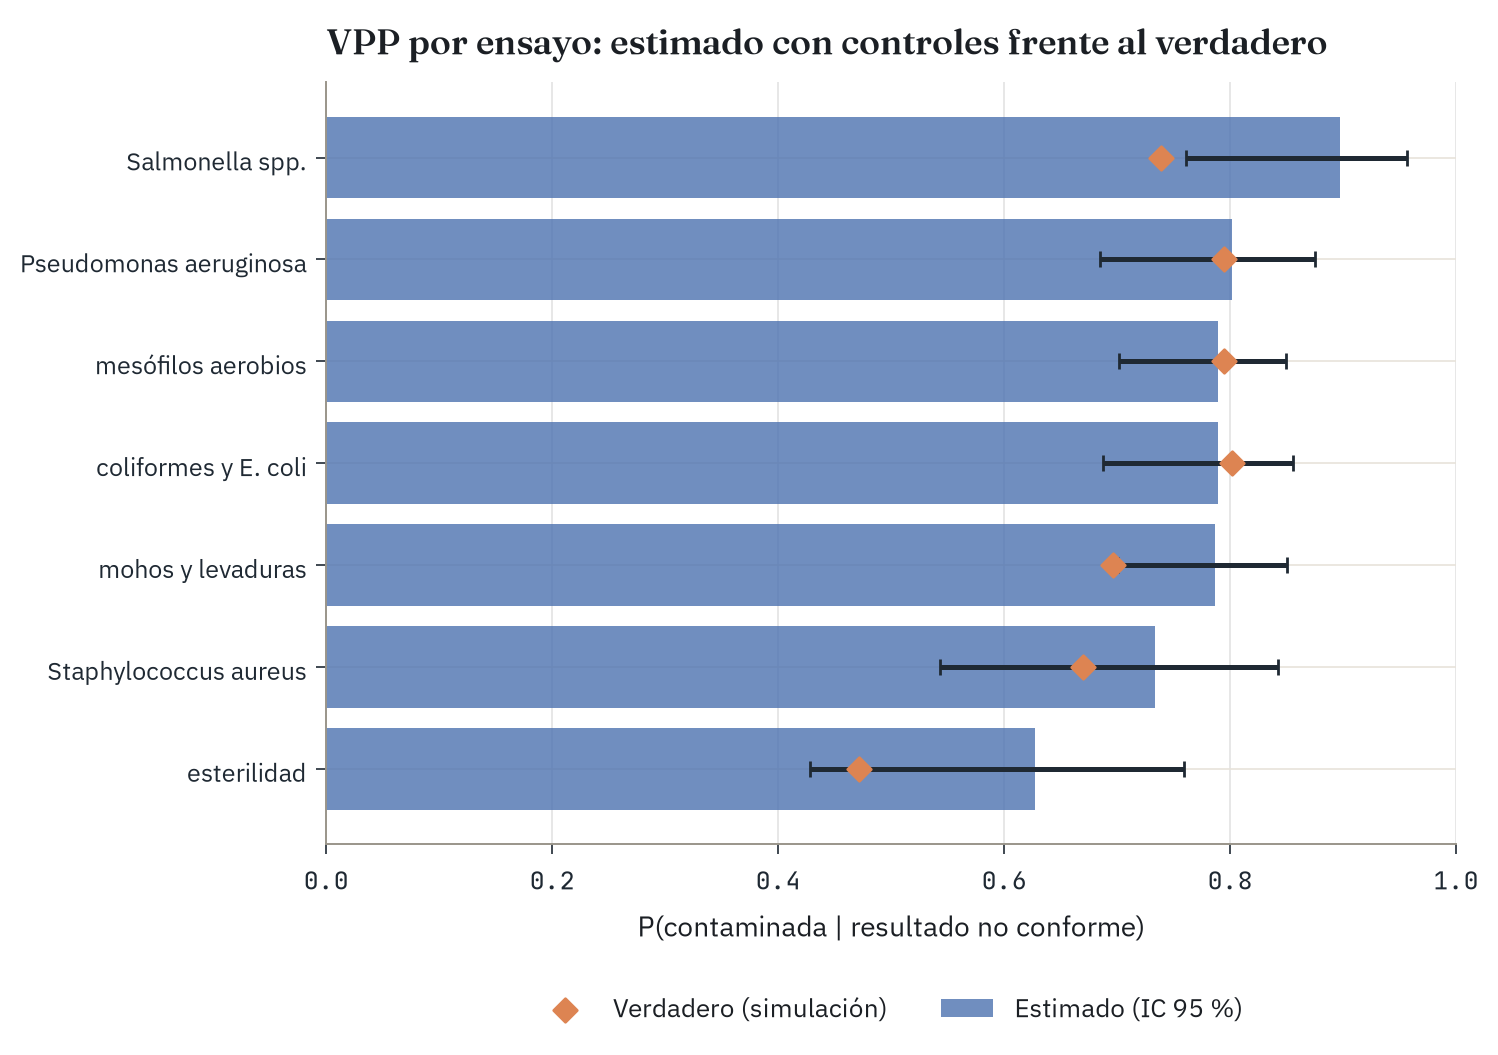
\includegraphics[width=\textwidth]{04_auditoria_vpp.png}
\caption{\textbf{Auditoría con la verdad de la simulación.} VPP por ensayo
estimado con los controles (barras con IC 95\,\%) frente al verdadero
(rombos): Los rombos que caen fuera del intervalo (\textit{Salmonella} y
mohos y levaduras) son los ensayos donde la estimación es optimista.}
\label{fig:auditoria}
\end{minipage}\hfill
\begin{minipage}[t]{0.49\textwidth}\centering
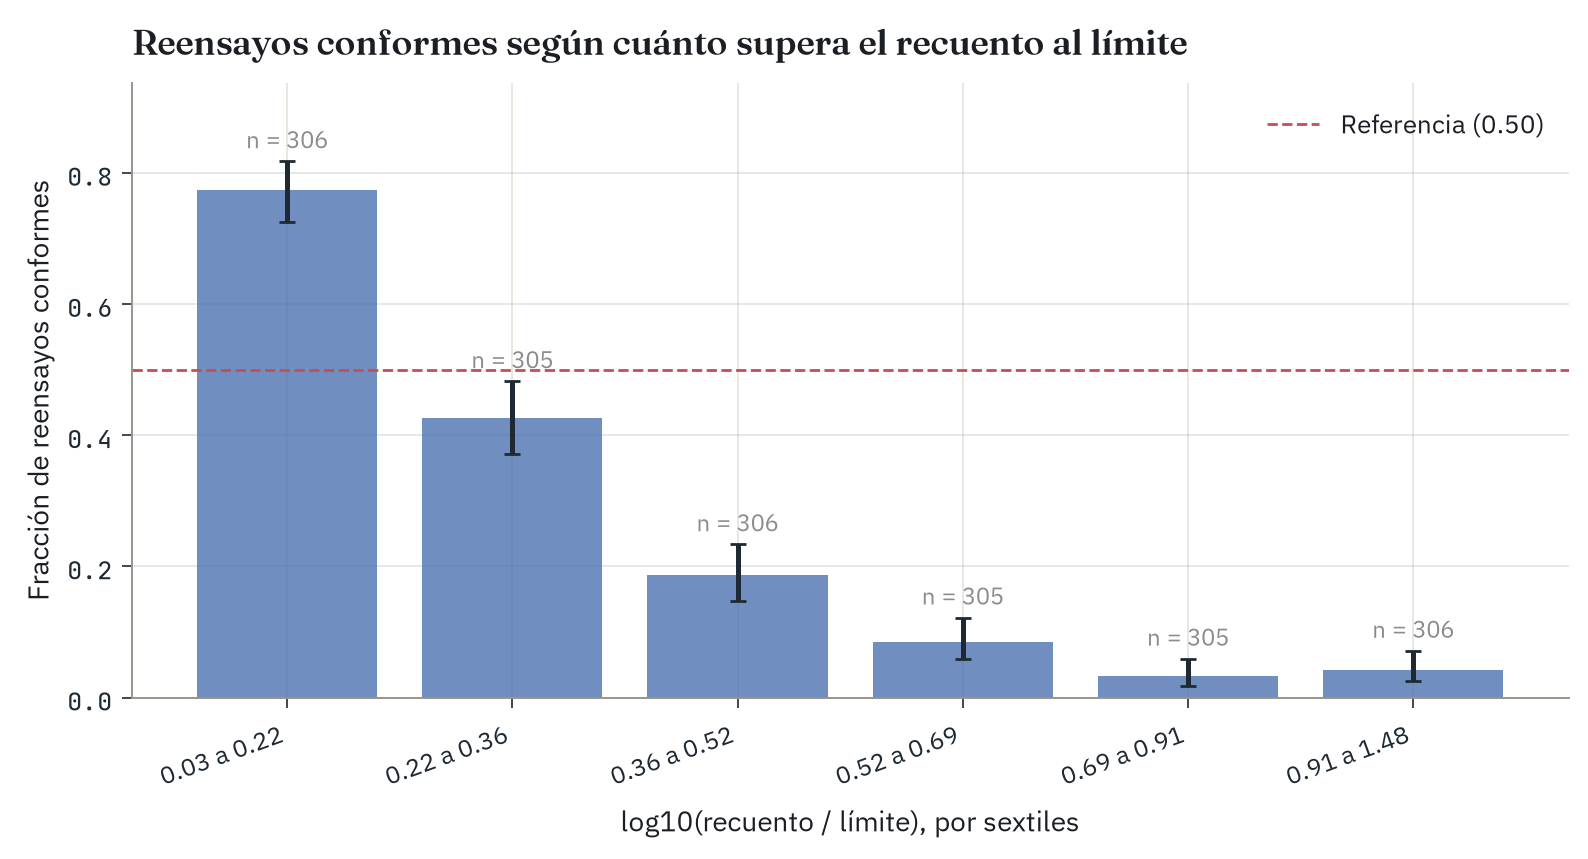
\includegraphics[width=\textwidth]{04_regla_reensayo.png}
\caption{Fracción de reensayos conformes según cuánto supera el recuento al
límite, por sextiles y con IC de Wilson: La caída es abrupta después del
primer sextil, que es el que define el borde de la regla de reensayo.}
\label{fig:regla}
\end{minipage}
\end{figure}
